We have a two-step approach for the coreference resolution task. The initial step involves single-document coreference resolution, where we utilize F-coref~\cite{otmazgin2022fcoref}. Subsequently, the second step focuses on cross-document coreference resolution, where we employ CDLM~\cite{caciularu-etal-2021-cdlm-cross}. In the context of single-document coreference resolution, F-coref emerges as a Python package designed for swift, precise, and user-friendly English coreference resolution. Drawing inspiration from s2e~\cite{kirstain-etal-2021-coreference}, F-coref introduces parallelism through batching, thereby reducing unnecessary computations like padded tokens. Similar to other neural coreference models, F-coref evaluates each pair of spans in the text for potential co-reference.

The architecture of F-coref encompasses three key components: (1) Longformer~\cite{beltagy2020longformer}, serving as a contextualized encoder; (2) a parameterized mention scoring function denoted as $f_m$; and (3) a parameterized pairwise antecedent scoring function labeled as $f_a$. To determine the coreference likelihood between any pair of spans, the model initiates by encoding the text through Longformer, resulting in vectors $x_1,...,x_n$. Subsequently, for each potential span $q$ = $(x_k, x_l)$, the mention scoring function $f_m(q)$ evaluates the probability of $q$ (the "query") being a mention. For a given pair of spans $c = (x_i, x_j)$ and $q = (x_k, x_l)$, where $c$ ("candidate") precedes $q$, the pairwise antecedent scoring function $f_a(c, q)$ assesses the likelihood of $c$ being an antecedent of $q$. In practical terms, to mitigate the complexity of $O(n^4)$, the antecedent function scores only the top $\lambda T$ spans with the highest mention scores (where $T$ represents the number of tokens). Ultimately, the final pairwise score for a coreference link between $c$ and $q$ comprises the scores indicating the likelihood of $q$ and $c$ being mentioned, along with the probability of $c$ being an antecedent of $q$:

\begin{equation}
  F(c,q) =
    \begin{cases}
      f_m(c)+f_m(q)+f_a(c,q) & \text{$c \neq \varepsilon$}\\
      0 & \text{$c = \varepsilon$},
    \end{cases}       
\end{equation}

where $\varepsilon$ is the null antecedent. The computation of $f_m$ and $f_q$ for the entire sequence can be efficiently batched.

In the cross-document coreference resolution task, we employ CDLM~\cite{caciularu-etal-2021-cdlm-cross} in Figure~\ref{fig:cdlm}, a pretraining approach designed for multi-document language modeling. This method incorporates two key concepts: (1) pretraining over sets of related documents with overlapping information and (2) pretraining utilizing a dynamic global attention pattern over masked tokens to reference the entire cross-text context. During pretraining over related documents, CDLM focuses on training the model on sets of documents that revolve around the same topic. This strategy aims to enhance the model's ability to understand cross-text mapping and alignment, contributing to improved unmasking.

To facilitate effective contextualization across multiple documents, CDLM leverages transformer models with linear scalability concerning input length, building upon the longformer model. The model processes input by concatenating related documents using dedicated document separator tokens, <doc-s> and </doc-s>, to demarcate document boundaries. Employing a masking strategy akin to BERT~\cite{devlin2019bert}, approximately 15\% of tokens in each training example are randomly chosen to be masked. However, CDLM's pretraining approach aims to predict each masked token by considering the entire document set and assigning them global attention weights. This unique approach enables the longformer to contextualize information across documents and handle long-range dependencies within documents. Ultimately, CDLM is employed to accomplish cross-document coreference resolution.

\begin{figure}
\centering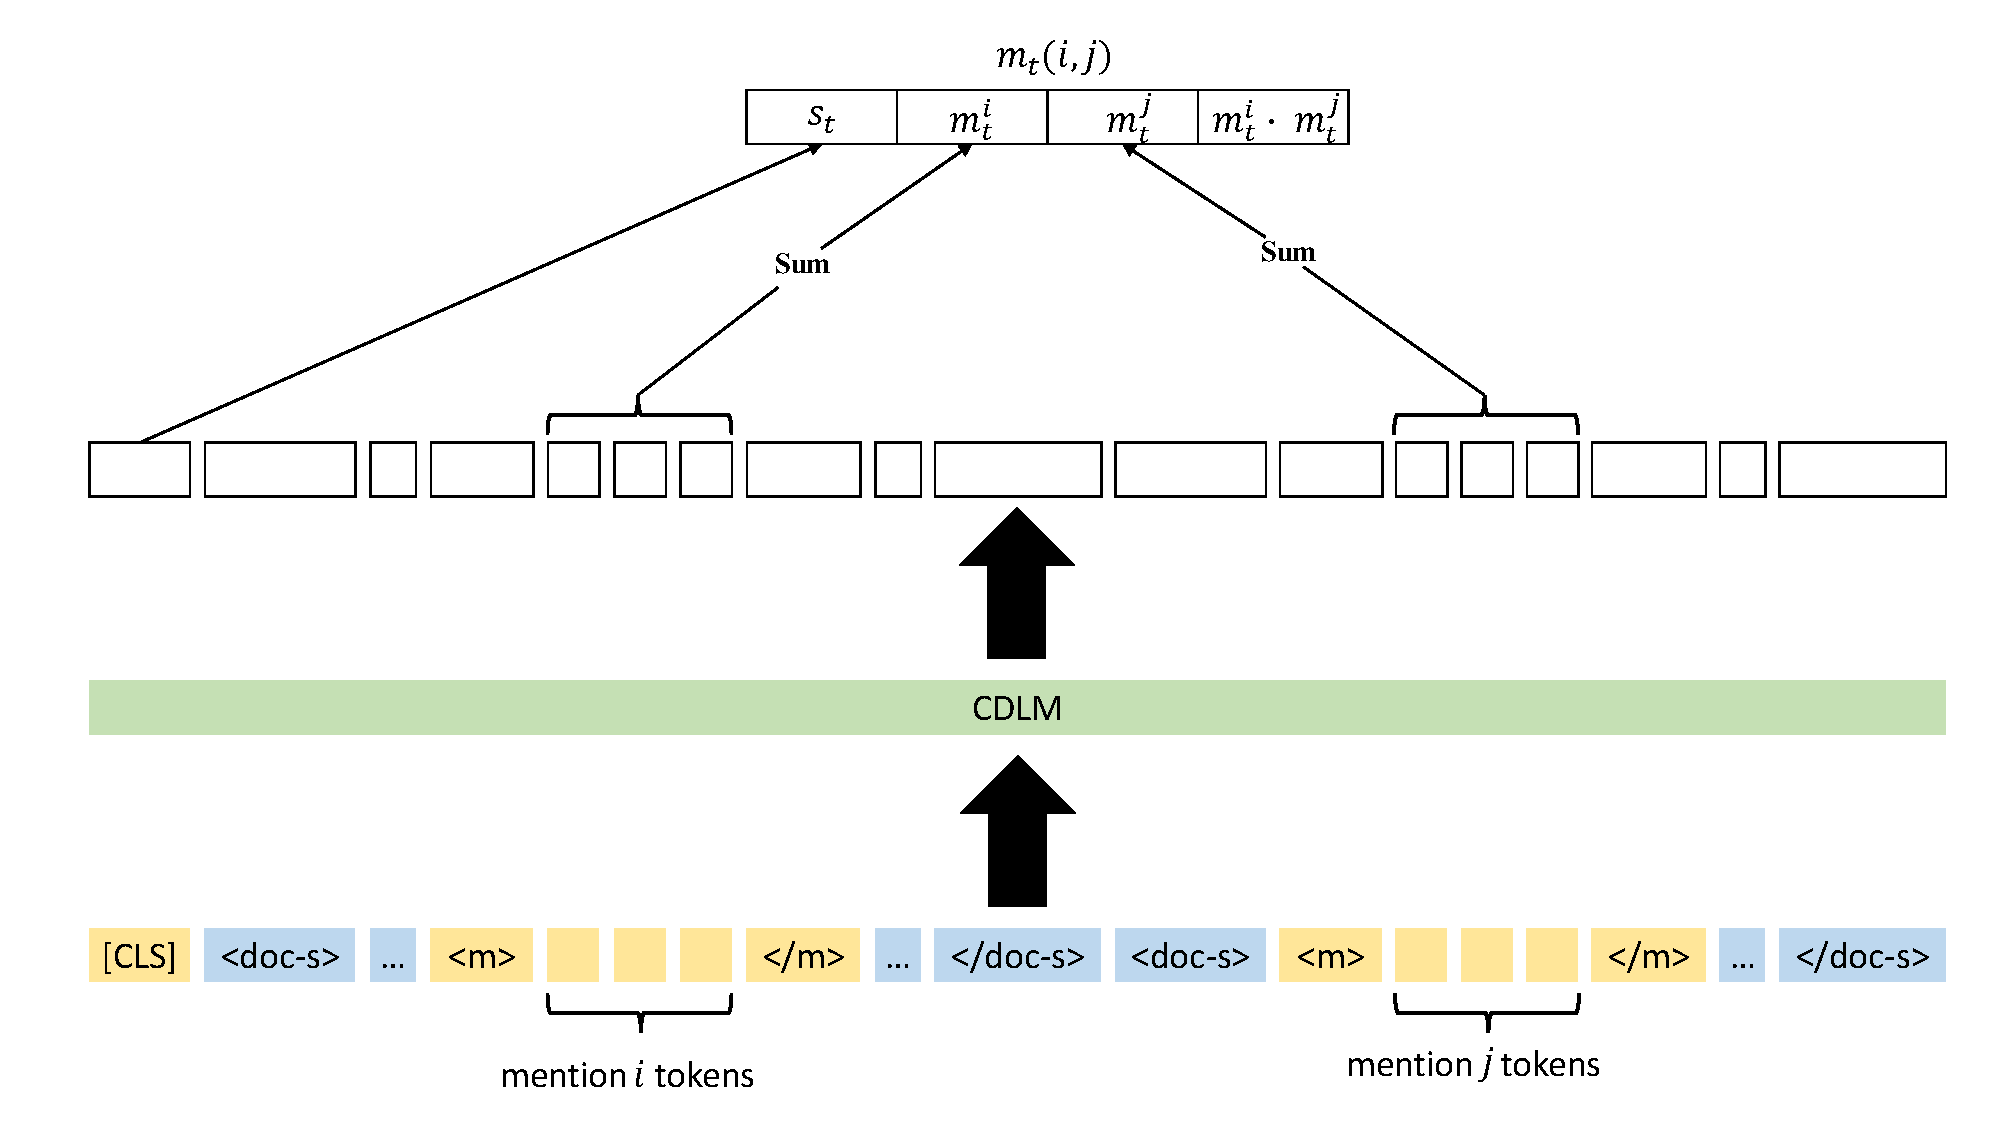
\includegraphics[width=\textwidth,height=\textwidth,keepaspectratio]{images/CDLM.pdf}
  \caption{The CDLM model utilizes pairwise mention representation for coreference resolution. $m_t^i$, $m_t^j$ and $s_t$ are the cross-document contextualized representation vectors for mentions $i$ and $j$, and of the [CLS] pairwise-mention representation. The tokens colored in yellow represent global attention, and the tokens colored in blue represent local attention.}
  \label{fig:cdlm}
\end{figure}

Upon completing coreference resolution in both single-document and cross-document scenarios, we integrate coreference relationships (:coref) into the KGs. These links signify the coreference relationships between the events and entities, aiding in the generation of claims that incorporate information from multiple documents. Figure~\ref{fig:visulization} illustrates the multimodal multi-document knowledge graph. Colors signify distinct documents, and the connection between nodes of different colors indicates coreference for a shared event or entity.

